\chapter{Organisation et structure}

\section{Organisation du sujet}

\subsection{Ordre de priorité}
L'organisation du projet a été soumit a un ordre de priorité car, comme cité dans "Mise en place du projet" (voir section \ref{sec:MEPprog}), certaines parties étaient nécessaires pour que d'autres fonctionnent ou puissent être amorcées :
\begin{itemize}
    \item La création de l'alphabet de notre L-Système (voir section \ref{sec:Alphabet}).
    \item La mise en place de la vérification des termes contenus dans les règles et l'axiome.
    \item La création du moteur de réécriture.
    \item La mise en place du Parser qui transforme le mot obtenu par le moteur de réécriture en une structure de données plus facilement lisible; afin d'être affichée par le moteur graphique.
    \item La création du moteur graphique.
    \item Et, pour faciliter l'utilisation de notre code, la création d'une interface.
\end{itemize}

\subsection{Repartition des tâches}
L'ordre de priorité étant fixé, nous sommes passé à la répartition des tâches. La création de l'alphabet s'est premièrement effectuée ensemble.
\\
Ensuite nous nous sommes répartis les tâches, Arthur et Quentin travaillant sur le Parser, Antonin et Thomas commençant à faire des recherches sur le moteur graphique que nous pourrions utiliser.
\\
Après cela, Quentin passa à la création du moteur graphique,aidé d'Arthur pour le déplacaement de la caméra, Antonin finalisant le Parser, Arthur et Thomas créant l'interface. Une fois toutes les parties principales créées et avancées, tout le monde a travaillé dans l'amélioration de celles-ci.
\\
Pour finir, la création du rapport s'est effectuée, elle aussi, en groupe.

\section{Structure du projet}
\begin{itemize}
    \item engine
    \begin{itemize}
        \item Rewrite: Moteur de réécriture
        \item Element, ElementProperties et Parser: voir section \ref{sec:parser}
    \end{itemize}
    \item screen
    \begin{itemize}
        \item Gl3d : Tout les objets relatifs a l'affichage 3d du L-Systeme, voir la section \ref{sec:interface3d}
        \item Main : Tout les objets relatifs au menu, voir la section \ref{sec:menu}
    \end{itemize}
    \item utils: contient l'objet Pair qui est essentiel au fonctionnement du projet
\end{itemize}

\begin{figure}[ht]
    \centering
    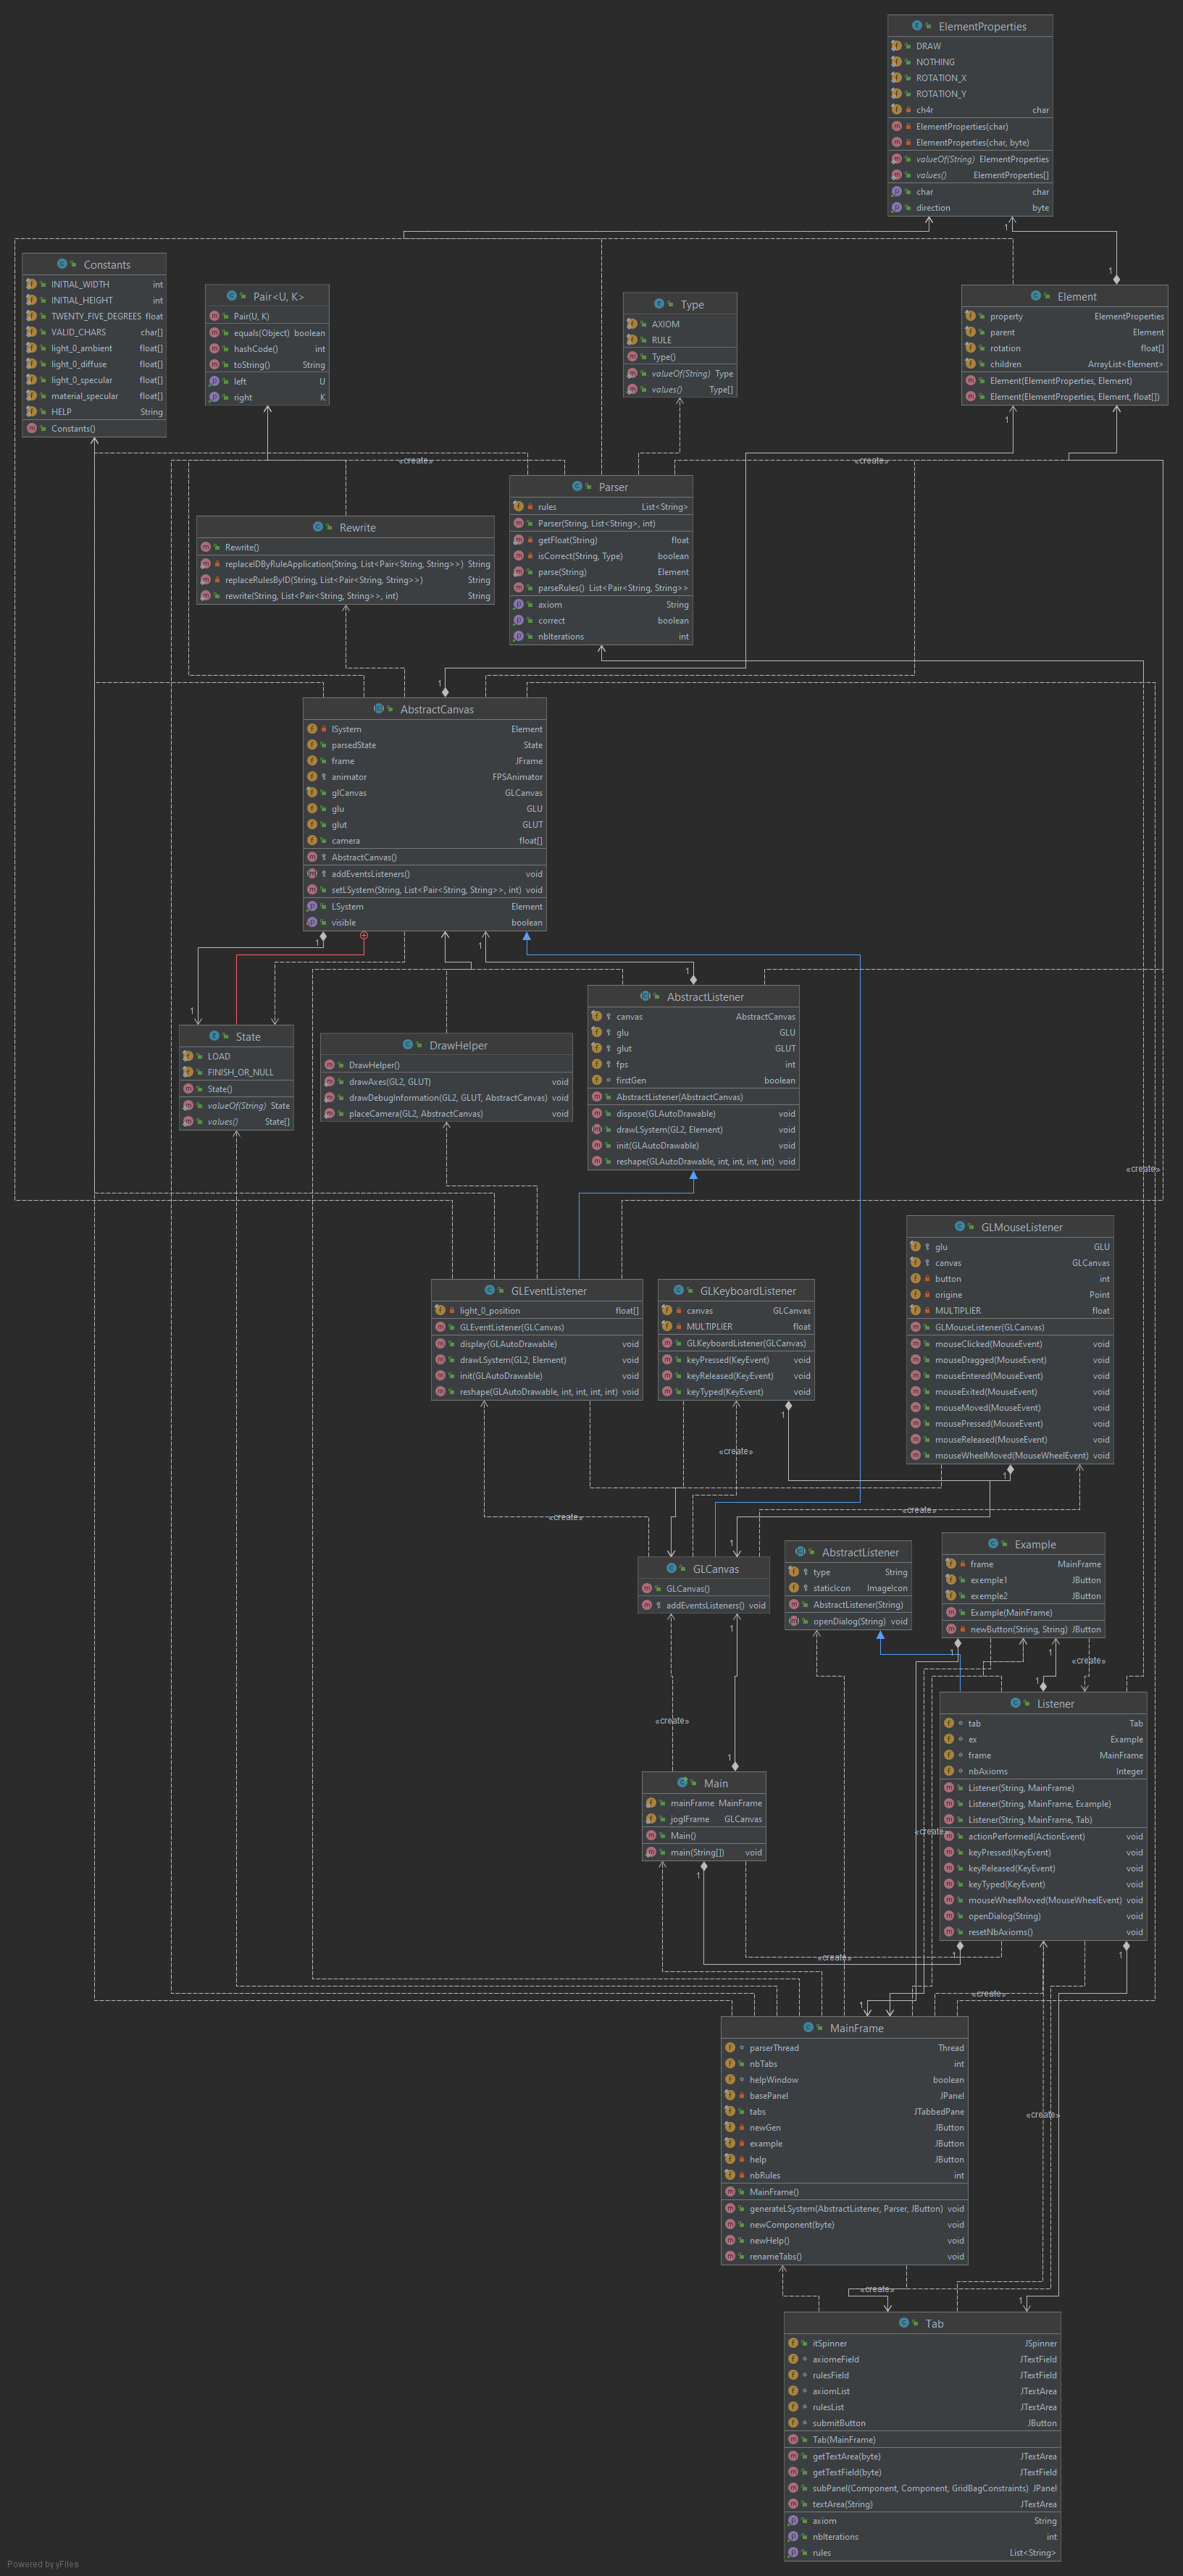
\includegraphics[width=0.7\linewidth]{pics/diagram.png}
    \caption{Diagramme de classe de notre projet}
    \label{fig:class_diagram}
\end{figure}

